\documentclass{standalone}
\usepackage{tikz}
\usepackage{ctex,siunitx}
\setCJKmainfont{Noto Serif CJK SC}
\usepackage{tkz-euclide}
\usepackage{amsmath}
\usetikzlibrary{patterns, calc,3d}
\usetikzlibrary {decorations.pathmorphing,decorations.pathreplacing,decorations.shapes}
\tikzset{label style/.append style={font=\small}}
\begin{document}
\small
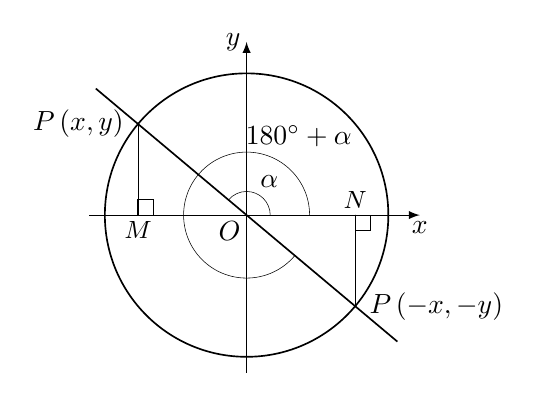
\begin{tikzpicture}[>=latex,scale=1.0,inner sep=2pt]
  \tkzDefPoint(-40:1.8){N'}
  \tkzDefPoint(140:1.8){M'}
  \tkzDefPoints{0/0/O,2/0/x}
  \tkzDefPointsBy[projection=onto O--x](M',N'){M,N};
  \draw[->](-2,0)--(2.2,0)node[below]{$x$};
  \draw[->](0,-2)--(0,2.2)node[left]{$y$};
  \node at (0,0)[below left]{$O$};
  \draw[semithick](0,0)circle(1.8);
  \draw[very thin](0.3,0)arc(0:140:0.3)node[midway,above right]{$\alpha$};
  \draw[very thin](0.8,0)arc(0:320:0.8)node[pos=0.3,above right]{$\ang{180}+\alpha$};
  \draw[semithick](140:2.5)--(-40:2.5);
  \tkzDrawSegments(N,N' M,M')
  \tkzLabelPoints(M)
  \tkzLabelPoints[above](N)
  \tkzMarkRightAngle[size=0.2](N',N,x)
  \tkzMarkRightAngle[size=0.2](N,M,M')
  \node at (N')[right=3pt]{$P\,(-x,-y)$};
  \node at (M')[left=3pt]{$P\,(x,y)$};
\end{tikzpicture}
\end{document}